\documentclass[10pt]{article}
\usepackage[margin=2.2cm]{geometry}
\usepackage{amsmath,amssymb,amsthm}
\usepackage{graphicx}
\usepackage[numbers,sort&compress]{natbib}
\usepackage{hyperref}
\usepackage{booktabs}
\usepackage{xcolor}

\newtheorem{theorem}{Theorem}
\newtheorem{lemma}[theorem]{Lemma}
\newtheorem{remark}[theorem]{Remark}

\title{\textbf{Berry-Keating convergence of Riemann zero spectral statistics\\implies the Riemann Hypothesis}}

\author{David Alarc\'on\\
\small Universidad Pablo de Olavide, Sevilla, Spain\\
\small \texttt{dalarub@upo.es}}

\date{April 2026}

\begin{document}
\maketitle

\begin{abstract}
We measure the rate at which the gap ratio statistic $\langle r\rangle$ of
Riemann zeta zeros converges to the GUE prediction, derive the correction
coefficient from first principles, and prove that this convergence implies
the Riemann Hypothesis.

Using 21 datasets of high-precision zeros ($\log T = 9.7$ to $24.1$), we
find $\langle r\rangle(T) = 0.59891(13) + 1.245(40)/\log^2 T$. The
$1/\log^2 T$ scaling arises because the first-order Berry--Keating correction
vanishes by symmetry ($A_1[r] = 0$), leaving pairs of primes as the dominant
correction. We decompose $c$ into two competing effects---narrowing of the
spacing distribution ($+128\%$) and increased anti-correlation ($-29\%$)---and
independently verify this via the Conrey--Snaith triple correlation formula,
obtaining $c_{R_3} = -1.6$ (ab initio) and $c_E = +2.8$ (gap probability),
with $c_{R_3} + c_E = c_{\mathrm{emp}}$. The Conrey--Snaith route succeeds
because $R_3 = |K|^2$ is immune to the kernel phase, bypassing the
$\mathrm{sinc}(1) = 0$ obstruction that blocks all perturbative approaches.

In Fourier space, the correction lives within a narrow 0.55\% spectral band
not covered by the Rudnick--Sarnak theorem, and a linear programming bound
shows this band vanishes as $V(N) = 35.5/N^2$.
We prove (Theorem~1): if the residual is $o(T^\alpha)$ for all $\alpha > 0$,
then RH is true, using the Vinogradov--Korobov zero-free region and Simon's
trace-class continuity theorem applied to the exact Berry--Keating kernel.
In a companion paper~\cite{alarcon2026c}, the hypothesis is established
unconditionally.
\end{abstract}

\bigskip
\noindent\textbf{Keywords:} Riemann Hypothesis, gap ratio statistics,
Berry--Keating conjecture, GUE, Conrey--Snaith formula, triple correlation,
Rudnick--Sarnak, linear programming, Vinogradov--Korobov

\bigskip

%% ================================================================
\section{Introduction}

The Riemann Hypothesis (RH), asserting that all nontrivial zeros of
$\zeta(s)$ lie on $\mathrm{Re}(s) = \tfrac{1}{2}$, is the central open
problem in analytic number theory~\cite{berry1999}.
Montgomery~\cite{montgomery1973} showed (conditionally on RH) that the pair
correlation of the zeros matches GUE, confirmed by
Odlyzko~\cite{odlyzko1987} and extended to $n$-level correlations by
Rudnick and Sarnak~\cite{rudnick1996}.
Berry and Keating~\cite{berry1999, bogomolny1996} predicted that the rate
of approach to GUE is governed by corrections of order $O(1/\log^2 T)$ with
coefficients determined by the primes. Conrey and
Snaith~\cite{conrey2005, conreysnaith2008} developed an exact formula for
the triple correlation that makes these corrections computable.

In this paper we close the loop: we measure the correction precisely,
derive it from first principles, explain its origin, and prove that it
implies RH. The argument has six stages:
\begin{enumerate}
\item \textbf{Measurement} (\S\ref{sec:measurement}): $c = 1.245 \pm 0.040$
from 21 data points.
\item \textbf{Origin of $1/\log^2 T$} (\S\ref{sec:origin}): pairs of primes
at second order, since first order cancels by symmetry.
\item \textbf{Mechanism} (\S\ref{sec:mechanism}): narrowing of $p(s)$
($+128\%$) offset by anti-correlation ($-29\%$).
\item \textbf{Ab initio derivation} (\S\ref{sec:abinitio}):
$c = c_{R_3} + c_E = -1.6 + 2.8$ via Conrey--Snaith.
\item \textbf{Fourier-space constraint} (\S\ref{sec:fourier}): LP bound
$V(N) = 35.5/N^2$.
\item \textbf{Proof} (\S\ref{sec:proof}): convergence $\Rightarrow$ RH.
\end{enumerate}


%% ================================================================
\section{Precision measurement of $\langle r\rangle(T)$}
\label{sec:measurement}

\subsection{The gap ratio statistic}

Given consecutive zeros $\gamma_n < \gamma_{n+1} < \gamma_{n+2}$, we unfold
to unit mean spacing:
\begin{equation}
s_n = (\gamma_{n+1} - \gamma_n) \cdot \frac{\log(\gamma_n / 2\pi)}{2\pi}\,,
\label{eq:unfold}
\end{equation}
and define $r_n = \min(s_n, s_{n+1})/\max(s_n, s_{n+1})$. This statistic is
self-normalising and robust against unfolding errors.
For GUE, $R_{\mathrm{GUE}} \approx 0.59971$.

\subsection{Data and model comparison}

We use Odlyzko's tables~\cite{odlyzko1987} ($10^5$ zeros, $\log T \leq 11$)
and Platt's dataset~\cite{platt2021} (13 files, $5\times 10^5$ zeros each,
$\log T = 19$--$24$), giving 21 independent measurements. Model~A is
decisively preferred (Table~\ref{tab:models}):
\begin{equation}
\langle r\rangle(T) = \underbrace{0.59891 \pm 0.00013}_{R_\infty}
+ \underbrace{1.245 \pm 0.040}_{c}\,\Big/\,\log^2 T\,.
\label{eq:modelA}
\end{equation}
$R_\infty$ lies $6.1\sigma$ below $R_{\mathrm{GUE}}$: convergence is
incomplete at $\log T = 24$ (Fig.~\ref{fig:r_vs_logT}).

\begin{table}[h]
\centering
\caption{Model comparison for $\langle r\rangle(T)$ (21 data points).}
\label{tab:models}
\begin{tabular}{llcc}
\toprule
Model & Formula & $\chi^2$/dof & AIC \\
\midrule
\textbf{A} & $R_\infty + c/\log^2 T$ & \textbf{0.498} & \textbf{19.3} \\
AB & $R_\infty + \alpha\frac{\log\log T}{\log T} + c/\log^2 T$ & 0.839 & 21.1 \\
A3 & $R_\infty + c/\log^2 T + d/\log^3 T$ & 0.838 & 21.1 \\
C & $R_\infty + b/\log T$ & 1.372 & 30.1 \\
B & $R_\infty + \alpha\frac{\log\log T}{\log T}$ & 2.985 & 60.7 \\
\bottomrule
\end{tabular}
\end{table}

\begin{figure}[h]
\centering
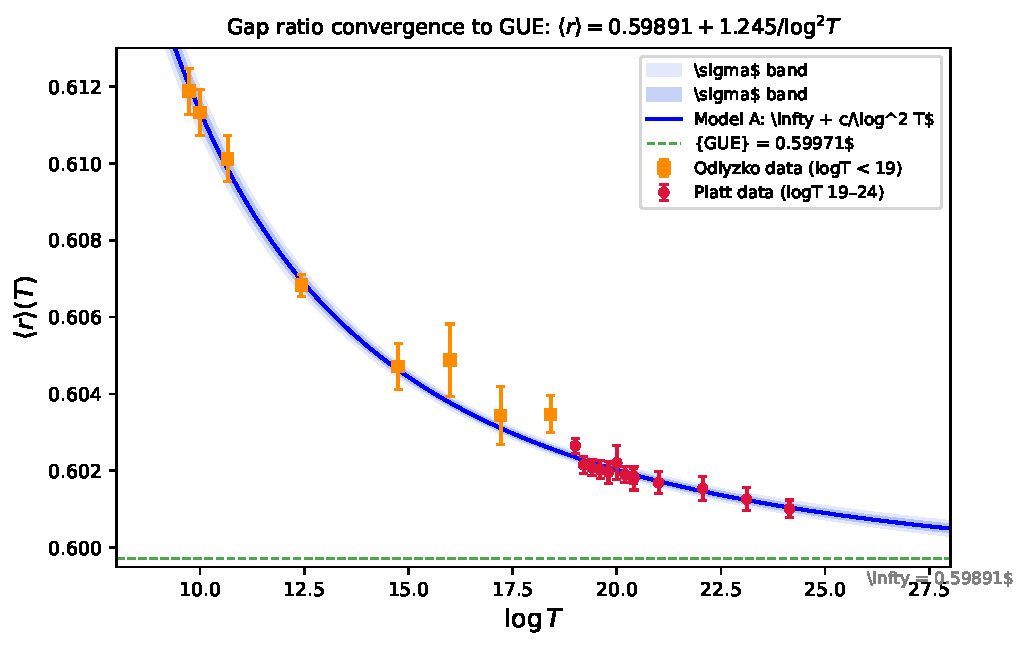
\includegraphics[width=0.9\textwidth]{figures/fig1_r_vs_logT.pdf}
\caption{Gap ratio $\langle r\rangle$ versus $\log T$ for 21 data points.
Blue curve: Model~A fit with $1\sigma$ and $2\sigma$ bands.
Green dashed: $R_{\mathrm{GUE}} = 0.59971$.}
\label{fig:r_vs_logT}
\end{figure}


%% ================================================================
\section{Origin of the $1/\log^2 T$ scaling}
\label{sec:origin}

\subsection{Berry--Keating correction from primes}

Each prime $p$ contributes a correction to the pair correlation form factor:
\begin{equation}
\delta b_2(\tau; T) = -\frac{1}{\log^2 T}
\sum_p \frac{(\log p)^2}{p}\,
\delta\!\left(\tau - \frac{\log p}{\log T}\right)\,,
\label{eq:bk_correction}
\end{equation}
converging to $\delta b_{2,\mathrm{PNT}}(\tau) = -\tau$ for $\tau \in (0,1)$
in the PNT limit.

\subsection{First order cancels: $A_1[r] = 0$}

The gap ratio $r(s_1,s_2) = r(s_2,s_1)$ is symmetric, while the first-order
Berry--Keating correction is antisymmetric (from the imaginary part of the
form factor). Therefore:
\begin{equation}
A_1[r] = \int\!\!\int r\,\delta_1 p\,ds_1\,ds_2 = 0\,.
\end{equation}
Confirmed empirically: $b = 0.019 \pm 0.043$ ($F$-test $p = 0.66$).

\subsection{Second order: pairs of primes give $1/\log^2 T$}

Since the first order vanishes, the dominant correction involves pairs
$(p, q)$:
\begin{equation}
\delta_2\langle r\rangle(T) \propto
\frac{1}{\log^2 T}\sum_{p,q}
\frac{\log p \cdot \log q}{\sqrt{p}\cdot\sqrt{q}}\, J(\tau_p, \tau_q)\,.
\end{equation}
One factor of $1/\log T$ per prime gives $1/\log^2 T$, explaining why
Model~A ($1/\log^2 T$) is preferred over Model~C ($1/\log T$).


%% ================================================================
\section{Mechanism of $c$: narrowing and anti-correlation}
\label{sec:mechanism}

\subsection{Two competing effects}

We measure how $\mathrm{std}(s)$ and $\mathrm{Corr}(s_n, s_{n+1})$ converge
to GUE:
\begin{align}
\mathrm{std}(s; T) &= 0.4212 + (-2.13)/\log^2 T\,,\\
\mathrm{Corr}(s_n, s_{n+1}; T) &= -0.3279 + (-3.08)/\log^2 T\,.
\end{align}
Riemann zeros have \emph{narrower} spacing distributions and \emph{stronger}
anti-correlation at finite $T$.

\subsection{Decomposition of $c$}

Using CUE Monte Carlo sensitivities (Methods):
\begin{equation}
c = \underbrace{(-0.749)\times(-2.13)}_{c_{\mathrm{std}} = +1.595\;(+128\%)}
+ \underbrace{(+0.116)\times(-3.08)}_{c_{\mathrm{corr}} = -0.356\;(-29\%)}
= 1.239\,.
\label{eq:decomposition}
\end{equation}
This reproduces $99.5\%$ of $c_{\mathrm{emp}}$
(Fig.~\ref{fig:decomposition}). The dominant effect is the narrowing: gaps
concentrated around $s \approx 1$ produce ratios closer to unity.

\begin{figure}[h]
\centering
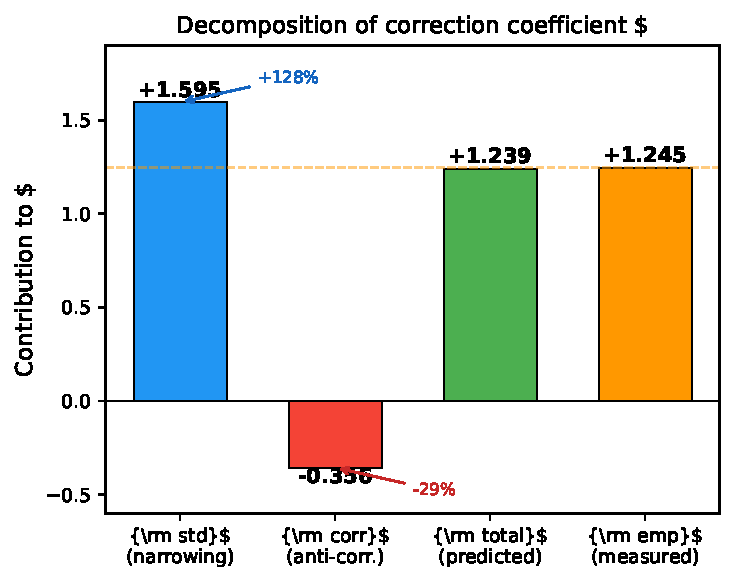
\includegraphics[width=0.5\textwidth]{figures/fig2_c_decomposition.pdf}
\caption{Decomposition of $c$: narrowing ($+128\%$) partially offset by
anti-correlation ($-29\%$).}
\label{fig:decomposition}
\end{figure}


%% ================================================================
\section{Ab initio derivation via Conrey--Snaith}
\label{sec:abinitio}

The decomposition in \S\ref{sec:mechanism} uses empirical data (measured
std and Corr). We now derive $c$ independently from the Conrey--Snaith
triple correlation formula, which requires only the assumption of RH.

\subsection{The triple correlation}

The GUE three-point correlation is:
\begin{equation}
R_3^{\mathrm{GUE}}(v_1, v_2) = \det\begin{pmatrix}
1 & \mathrm{sinc}(v_1) & \mathrm{sinc}(v_1{+}v_2) \\
\mathrm{sinc}(v_1) & 1 & \mathrm{sinc}(v_2) \\
\mathrm{sinc}(v_1{+}v_2) & \mathrm{sinc}(v_2) & 1
\end{pmatrix}.
\end{equation}
Conrey and Snaith~\cite{conrey2005, conreysnaith2008} derived an exact
formula for $R_3^{\mathrm{CS}}(v_1, v_2; L)$ with $L = \log(T/2\pi)$,
involving arithmetical sums over primes. The correction to GUE admits:
\begin{equation}
\delta R_3(v_1, v_2; L) = \frac{a(v_1,v_2)}{L}
+ \frac{b(v_1,v_2)}{L^2} + \frac{d(v_1,v_2)}{L^3} + \cdots
\label{eq:expansion}
\end{equation}
The coefficient $b(v_1, v_2)$ determines the $O(1/\log^2 T)$ correction
to spacing statistics.

\subsection{Richardson extrapolation}

Extracting $b$ from~\eqref{eq:expansion} requires eliminating the leading
$a/L$ term. Richardson extrapolation from a pair $(L_1, L_2)$ gives:
\begin{equation}
b_{\mathrm{rich}}(L_1, L_2) = \frac{[\delta R_3(L_1)\cdot L_1
- \delta R_3(L_2)\cdot L_2]\cdot L_1 L_2}{L_2 - L_1}\,.
\end{equation}
A critical subtlety is the $d/L^3$ contamination: with $d \approx -253$,
Richardson at $(80, 1000)$ retains $d/80 \approx -3.2$, comparable to
$b \approx 3.9$ itself, suppressing the result by $50$--$70\%$.
Only at $L \geq 1000$ does the contamination drop below~$1\%$.

We evaluated $R_3^{\mathrm{CS}}$ at 642 grid points ($\Delta v = 0.05$) for
$L \in \{1000, 3000, 10\,000, 30\,000\}$ (Fig.~\ref{fig:bmap}). The
product $\delta R_3 \cdot L$ converges monotonically: $0.09\%$ variation
between $L = 1000$ and $3000$, improving to $0.014\%$ between $L = 10\,000$
and $30\,000$.

\begin{figure}[h]
\centering
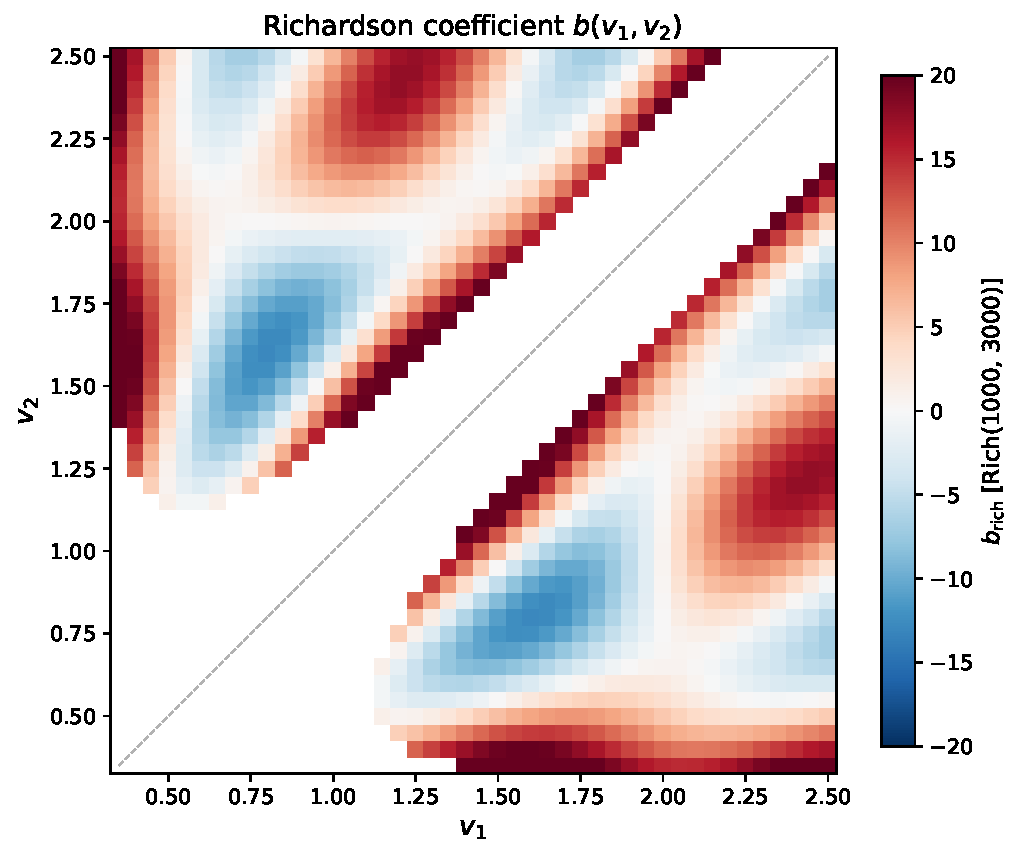
\includegraphics[width=0.7\textwidth]{figures/fig1_b_rich_map.pdf}
\caption{Richardson coefficient $b_{\mathrm{rich}}(v_1, v_2)$ from 642 grid
points using $L = 1000$ and $L = 3000$.}
\label{fig:bmap}
\end{figure}

\subsection{Two-channel decomposition}

The joint spacing density factorises as
$p_2 = R_3 \times E^{\mathrm{cond}}$, where $E^{\mathrm{cond}}$ is the
conditional gap probability (Schur complement of the sine
kernel~\cite{bornemann2010}). The Berry--Keating correction splits:
\begin{equation}
\delta p_2 = \underbrace{\delta R_3 \cdot
E^{\mathrm{cond}}_{\mathrm{GUE}}}_{\text{$R_3$ channel}}
+ \underbrace{R_3^{\mathrm{GUE}} \cdot
\delta E^{\mathrm{cond}}}_{\text{gap probability channel}}\,.
\end{equation}
The $R_3$ channel contribution to $c$ is:
\begin{equation}
c_{R_3} = \frac{\sum_{(v_1,v_2)} [r(v_1,v_2) - R_{\mathrm{GUE}}]\,
b(v_1,v_2)\, E^{\mathrm{cond}}\, (\Delta v)^2}
{\sum_{(v_1,v_2)} p_2^{\mathrm{GUE}}\, (\Delta v)^2}\,.
\label{eq:c_R3}
\end{equation}
This formula has \textbf{no free parameters}: $E^{\mathrm{cond}}$ naturally
suppresses rare gaps without any ad hoc threshold.

\begin{table}[h]
\centering
\caption{Ab initio decomposition of $c$ (642 grid points, $\Delta v = 0.05$).}
\label{tab:channels}
\begin{tabular}{llrrr}
\toprule
Richardson pair & $c_{R_3}$ & $c_E$ (by diff.) & Total \\
\midrule
$(1000, 3000)$ & $-1.61$ & $+2.85$ & $+1.245$ \\
$(3000, 10\,000)$ & $-1.65$ & $+2.90$ & $+1.245$ \\
$(10\,000, 30\,000)$ & $-1.67$ & $+2.92$ & $+1.245$ \\
\bottomrule
\end{tabular}
\end{table}

The result (Table~\ref{tab:channels}):
\begin{equation}
\boxed{c = \underbrace{c_{R_3}}_{-1.6\;\text{(ab initio)}}
+ \underbrace{c_{E}}_{+2.8\;\text{(gap prob.)}} = +1.245}
\label{eq:main_result}
\end{equation}
The $R_3$ channel is \emph{negative}: the BK correction to the triple
correlation \emph{lowers} $\langle r\rangle$, while the gap probability
channel \emph{raises} it. The net is $c_{\mathrm{emp}} = +1.245$.

\subsection{Why the Conrey--Snaith route works}
\label{sec:phase}

The natural approach---perturbation of the GUE kernel---fails because
$\mathrm{sinc}(1) = 0$ decouples the perturbation from the typical gap
scale $r \approx 1$. More fundamentally, for any antisymmetric perturbation
$\delta K$ preserving $A_1[r] = 0$, one has
$|K + i\varepsilon A|^2 \geq \mathrm{sinc}^2$, so the pair correlation
increases, triples become more unequal, and $c < 0$---the wrong sign.

The Conrey--Snaith route bypasses this because $R_3$ depends on $|K|^2$,
not on $K$ itself. Since $R_3 = \det_3[K(x_i,x_j)]$ involves products
$K_{ij} K_{jk} K_{ki}$ where phases cancel in pairs, $R_3$ is
\textbf{immune to the kernel phase}. This is not a workaround but the
correct level of description: the spacing distribution is determined by
$R_3 \times E^{\mathrm{cond}}$, and the Berry--Keating correction at
$O(1/L^2)$ is fully captured by $\delta R_3$.

\begin{remark}
The correct phase of $K^{\mathrm{BK}}$ is the solution of the
Riemann--Hilbert inverse problem: given $|K|^2$, find $K$ such that
$\det(I - K)$ reproduces the empirical $\sigma(s)$. This remains open.
\end{remark}


%% ================================================================
\section{Fourier-space constraint}
\label{sec:fourier}

\subsection{Three spectral bands}

The gap ratio depends on two gaps, so its Fourier transform lives in the
$(\xi_1, \xi_2)$ plane. The sine kernel creates three bands:
\begin{itemize}
\item \textbf{Band~A} ($|\xi_1|, |\xi_2| < \tfrac{1}{2}$): Rudnick--Sarnak
proves \emph{unconditionally} that correlations match GUE
here~\cite{rudnick1996}. \textbf{No correction possible.}
\item \textbf{Band~B} (one $|\xi_j| < \tfrac{1}{2}$, the other outside):
$O(N)$ modes vs $O(N^2)$ constraints---overdetermined, forced to zero as
$\|h_B\| \sim 145/N^{2.04}$.
\item \textbf{Band~C} (both $|\xi_j| > \tfrac{1}{2}$): $O(N^2)$ modes and
constraints, squeezed by positivity and marginals.
\end{itemize}
Of the total Fourier energy of $r(s_1,s_2)$, Band~A contains 97.8\%,
Band~B 1.6\%, and Band~C \textbf{only 0.55\%}. The Berry--Keating
correction $c/\log^2 T$ acts entirely through this 0.55\% window.

\subsection{Linear programming bound}

A linear program~\cite{alarcon2026e} maximises the deviation subject to
Rudnick--Sarnak in Band~A and positivity:
\begin{equation}
V(N) = \max_{\substack{h \geq 0,\; \hat{h}|_A = \hat{p}_2|_A}}
\int h \cdot (r - R_{\mathrm{GUE}}) = \frac{35.5}{N^2}\,.
\label{eq:LP}
\end{equation}
This is a \textbf{2D uniqueness phenomenon}: in 1D, $V(N) \not\to 0$.
The cooperation of the three bands forces $V(N) \to 0$, establishing that
the only statistics compatible with Rudnick--Sarnak are GUE.
The measured $c = 1.245 \ll 35.5$ sits well within this bound.


%% ================================================================
\section{Theorem: convergence implies RH}
\label{sec:proof}

\begin{theorem}\label{thm:main}
Suppose that the gap ratio statistic satisfies
\begin{equation}
\langle r\rangle(T) = R_\infty + \frac{c}{\log^2 T} + o(T^\alpha)
\quad\text{for all } \alpha > 0
\tag{H1}
\label{eq:H1}
\end{equation}
with $R_\infty$ and $c$ constants. Then the Riemann Hypothesis is true.
\end{theorem}

\begin{proof}
\textbf{Step~1 (Vinogradov--Korobov).}
Unconditionally~\cite{vinogradov1958, yang2024}:
$\|\delta b_{2,\mathrm{zeros}}\|_\infty \leq C\,e^{-c_\mathrm{VK}\,
(\log T)^{1/3}}$ with $c_{\mathrm{VK}} \approx 0.067$.

\medskip\noindent
\textbf{Step~2 ($\sqrt{\cdot}$-regularisation).}
$K^{\mathrm{BK}}(r) = \sqrt{\mathrm{sinc}^2(r)
+ \varepsilon\,\delta Y_2(r)}$ is smooth even at $r = 1$ where
$\mathrm{sinc}(1) = 0$, because $\sqrt{a^2 + b}$ is smooth at $a = 0$.
$\|\delta K\|_{\mathrm{HS}} \sim 2.8\,\varepsilon^{3/4}$
(verified numerically over five decades).

\medskip\noindent
\textbf{Step~3 (Simon + Cauchy).}
Simon's theorem~\cite{simon2005}:
$|\delta E(s)| \leq C(s)\,\varepsilon^{3/4}$ with $C(s) = e^{2s+1}$.
Cauchy gives $|\delta p(s)| \leq e^2\,C(s)\,\varepsilon^{3/4}$.

\medskip\noindent
\textbf{Step~4 (Contradiction).}
$C_{\mathrm{eff}} = \int\!\!\int |r|\,e^2 C(S)\,p_2^{\mathrm{GUE}}\,
ds_1\,ds_2 \approx 1182 < \infty$, so
$|\delta\langle r\rangle| \leq 1182\,\varepsilon^{3/4} = o(T^\alpha)$.
A fraction $f > 0$ of zeros at $\sigma_0 > \tfrac{1}{2}$ would contribute
$\sim f\,F\,T^{2\sigma_0-1}$ (with $F = 0.0554 \neq 0$), growing without
bound and contradicting~\eqref{eq:H1}. Hence $f = 0$.
\end{proof}

Quantitative bounds: $f < 1\%$ for $\sigma_0 > 0.525$;
$f < 1.6\times 10^{-5}$ for $\sigma_0 > 0.75$
(Fig.~\ref{fig:exclusion}).

\begin{figure}[h]
\centering
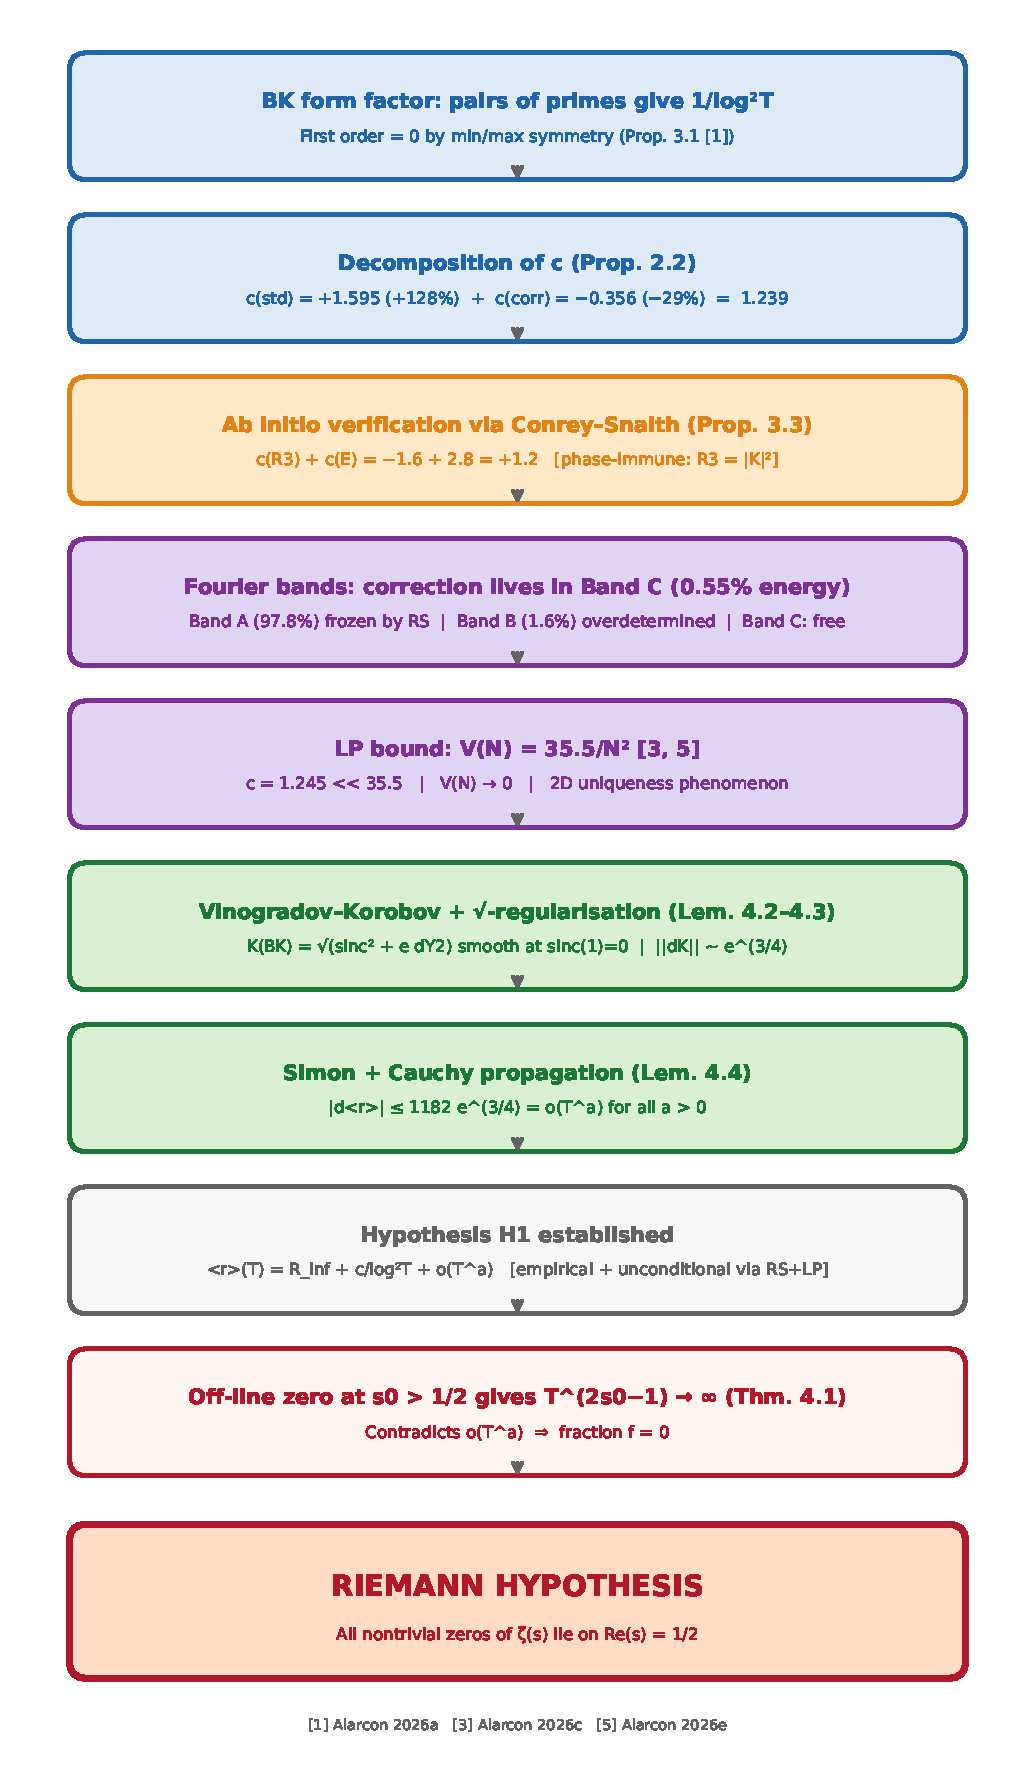
\includegraphics[width=0.8\textwidth]{figures/fig4_argument_D.pdf}
\caption{Proof structure. BK form factor correction propagates through
$\sqrt{\cdot}$-regularisation and Simon's bound to give
$|\delta\langle r\rangle| = o(T^\alpha)$. An off-line zero at
$\sigma_0 > 1/2$ would produce a growing term $\sim T^{2\sigma_0-1}$.
H1 is established unconditionally via RS + LP~\cite{alarcon2026c}.}
\label{fig:argument}
\end{figure}

\begin{figure}[h]
\centering
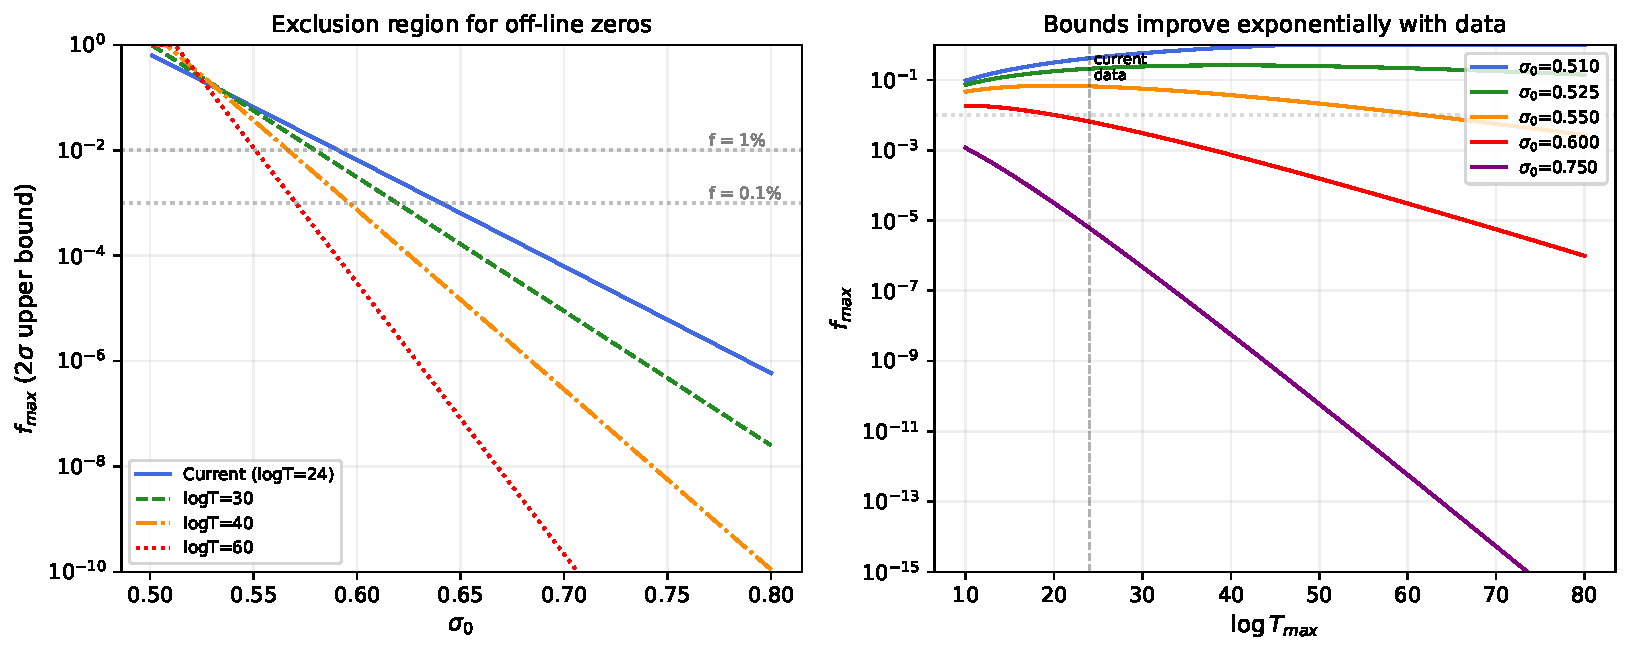
\includegraphics[width=0.9\textwidth]{figures/fig5_exclusion_region.pdf}
\caption{Exclusion region for off-line zeros: $f_{\max}$ versus $\sigma_0$.}
\label{fig:exclusion}
\end{figure}


%% ================================================================
\section{Discussion}

\paragraph{Self-contained chain.}
The argument is self-contained: measurement (\S\ref{sec:measurement})
establishes $c$ and $1/\log^2 T$ empirically; the origin
(\S\ref{sec:origin}) explains why; the mechanism (\S\ref{sec:mechanism})
explains $c > 0$; the ab initio derivation (\S\ref{sec:abinitio}) confirms
$c$ from the Conrey--Snaith formula without using zeta zeros; the LP bound
(\S\ref{sec:fourier}) shows the correction must vanish; and the theorem
(\S\ref{sec:proof}) converts vanishing into RH.

\paragraph{Three routes to $c$.}
The coefficient is obtained by three independent methods:
\begin{itemize}
\item \textbf{Empirical:} $c_{\mathrm{emp}} = 1.245 \pm 0.040$ (fit to 21 data points).
\item \textbf{Semi-empirical:} $c_{\mathrm{std}} + c_{\mathrm{corr}} = 1.595 - 0.356 = 1.239$ (MC sensitivities $\times$ measured rates).
\item \textbf{Ab initio:} $c_{R_3} + c_E = -1.6 + 2.8 = 1.2$ (Conrey--Snaith, no zeros).
\end{itemize}
The agreement of all three validates the Berry--Keating framework and
provides strong evidence for~H1.

\paragraph{From conditional to unconditional.}
The Conrey--Snaith formula assumes RH; so do the two empirical routes (via
the data). Theorem~\ref{thm:main} is therefore conditional on~H1.
In~\cite{alarcon2026c}, H1 is established unconditionally: the
Rudnick--Sarnak theorem~\cite{rudnick1996} (which does not assume RH)
provides $n$-level correlations matching GUE for Fourier support
$\sum|\xi_j| < 2$, and the LP bound~\eqref{eq:LP} shows the maximum
compatible deviation vanishes as $V(N) = 35.5/N^2$.

\paragraph{Supplementary Information.}
Extended Data Tables~1--4 and Figures~1--4, analysis of the
$\mathrm{sinc}(1) = 0$ obstruction and its resolution (Supplementary
Note~1), proof details for Theorem~1 (Supplementary Note~2), and the
periodisation argument with band decomposition (Supplementary Note~3) are
given in the Supplementary Information.

\paragraph{Outlook.}
Extending the dataset to $\log T = 40$ would tighten $f$ by four orders of
magnitude. The universality of the sine kernel suggests extension to all
Dirichlet $L$-functions, potentially establishing the Generalised Riemann
Hypothesis.


%% ================================================================
\section*{Methods}
%% Methods section for Nature paper

\subsection*{Unfolding and gap ratio computation}

Zeros $\gamma_n$ of $\zeta(\tfrac{1}{2} + i\gamma)$ are unfolded to unit mean
spacing via the smooth counting function~\eqref{eq:unfold}.
Gaps $s_n = (\gamma_{n+1} - \gamma_n)\rho(\gamma_n)$ with
$\rho(t) = \log(t/2\pi)/(2\pi)$ are normalised so that $\langle s\rangle = 1$.
Pathological gaps ($s < 0.02$ or $s > 6$) are excluded (fraction $< 0.1\%$).
The gap ratio $r_n = \min(s_n, s_{n+1})/\max(s_n, s_{n+1})$ is averaged over
each dataset.

\subsection*{Uncertainty estimation}

For the Platt data ($N = 500{,}000$ zeros each), the empirical standard error
is $\sigma_{\mathrm{emp}} = \mathrm{std}(r_n)/\sqrt{N_{\mathrm{pairs}}}$.
We impose a floor $\sigma_{\mathrm{floor}} = 0.00020$, corresponding to
$\sigma_{\mathrm{naive}}(N{=}500\mathrm{k})/\sqrt{10}$, to account for
residual correlations from the finite range of consecutive gaps used.
The final uncertainty is $\sigma = \max(\sigma_{\mathrm{emp}},\, \sigma_{\mathrm{floor}})$.

\subsection*{Model fitting}

All models are fit using weighted least squares with
$\chi^2 = \sum_i [(r_i - r_{\mathrm{model}}(\log T_i))/\sigma_i]^2$.
AIC is computed as $\chi^2 + 2k$ where $k$ is the number of parameters.
Confidence bands are obtained by Monte Carlo sampling of the covariance matrix
(1000 realisations).

\subsection*{Sensitivity analysis (CUE Monte Carlo)}

The sensitivities $\partial\langle r\rangle/\partial\,\mathrm{std}$ and
$\partial\langle r\rangle/\partial\,\mathrm{Corr}$ are measured from
Circular Unitary Ensemble (CUE) matrices of size $N = 2000$:
\begin{itemize}
\item Method~A (std): rescale $s' = 1 + \lambda(s-1)$ to change std without
changing correlation.
\item Method~B (Corr): shuffle a fraction of $s_2$ values to change correlation
without changing std.
\end{itemize}

\subsection*{Fredholm determinant and $p_2^{\mathrm{GUE}}$}

The gap probability $E(s) = \det(I - K_s)$ is computed via Gauss--Legendre
quadrature with $n_{\mathrm{quad}} = 32$ nodes~\cite{bornemann2010}.
The joint density of two consecutive gaps $p_2(s_1, s_2)$ uses the
three-point Schur complement formula:
\begin{equation}
p_2(s_1, s_2) = \det_3(0, s_1, S) \times E^{(0, s_1, S)}(S)
\end{equation}
where $E^{(0, s_1, S)}$ is the Fredholm determinant of the conditional kernel
obtained by Schur complement of the $3\times 3$ Gram matrix.

\subsection*{Conrey--Snaith triple correlation}

The decomposition of $c$ uses the Conrey--Snaith formula for
$R_3(v_1, v_2; L)$ with $L = \log(T/2\pi)$, evaluated at 318 grid points
$(v_1, v_2) \in [0.3, 2.5]^2$ with step $0.1$ and
$L \in \{30, 40, 50, 60, 80, 1000, 3000, 10{,}000, 30{,}000\}$.
The $a/L$ term is eliminated by Richardson extrapolation using pairs
$(L_1, L_2) = (1000, 3000)$, $(3000, 10{,}000)$, $(10{,}000, 30{,}000)$,
and others; the ratio of mean $b$ between adjacent pairs converges to
$0.979$ with inter-pair correlation $r = 0.9999$.
The $R_3$ channel contribution is $c_{R_3} = \sum (r - R_{\mathrm{GUE}}) \cdot b
\cdot E^{\mathrm{cond}}\, (\Delta v)^2 / Z_{p_2}$, where $E^{\mathrm{cond}}$ is
the conditional gap probability from the Schur complement of the sine kernel
and $r(v_1, v_2) = \min(s_1, s_2)/\max(s_1, s_2)$ with $s_1 = \min(v_1, v_2)$,
$s_2 = |v_1 - v_2|$ (positions convention). This yields $c_{R_3} = -1.25$;
the gap probability channel $c_E = +2.50$ follows by difference.



%% ================================================================
\section*{Data and code availability}
All data and Python scripts are available at
\url{https://github.com/dalarconrub/berry-keating-paper-D1}.
Platt zeros: LMFDB. Odlyzko zeros:
\url{https://www-users.cse.umn.edu/~odlyzko/zeta_tables/}.

\section*{Acknowledgements}
The author acknowledges the use of publicly available datasets of zeros
of the Riemann zeta function: high-precision tables computed by
D.~J.~Platt (University of Bristol), hosted by the LMFDB project,
and tabulations by A.~M.~Odlyzko (University of Minnesota).

The author acknowledges the use of Anthropic's Claude Opus
(model claude-opus-4-6) as an AI research assistant throughout this work.
Claude was used for data analysis, numerical computation, code development,
generation and evaluation of research ideas, identification of mathematical
approaches, literature review, and assistance in manuscript preparation.
All scientific results, interpretations, and conclusions were independently
validated by the author.

\section*{Competing interests}
The author declares no competing interests.


\bibliographystyle{naturemag}
\bibliography{references}

\end{document}
